\subsection{Arricchimento di Strutture Dati}

Vedremo due esempi, uno per gli RB-trees, e un altro per gli ABR.
\begin{itemize}[noitemsep]
    \item \emph{Statistiche d'ordine} (\ref{statistichedordine})
    \item \emph{Interval Trees} (\ref{intervaltrees})
\end{itemize}

\subsubsection{Statistiche d'ordine} \label{statistichedordine}
Struttura che parte da un RB-tree. Aggiungo:
\begin{itemize}
    \item \texttt{Select(T,i)} $\equiv$ nodo $x$ che occuperebbe la posizione $i$
        nei nodi ordinati per chiave (in una \emph{visita simmetrica});
    \item \texttt{Rank(T,x)} $\equiv$ posizione $i$ (in una \emph{visita simmetrica}) 
        che occupa il nodo $x$. 
\end{itemize}

Per implementare queste due procedure, ho bisogno di un nuovo campo dati. 
Aggiungo il campo 
$$x.size = \# \text{nodi radicati nel sottoalbero } T_x$$ 
Valgono
\begin{itemize}[label=,noitemsep]
    \item $T.nil.size = 0$
    \item $x.size = x.left.size + x.right.size + 1$
\end{itemize}

\paragraph{Esempio} In ogni nodo, tra le parentesi
è riportato la $size$ di quel nodo. Ricordiamo che i nodi $nil$ ($T.nil$)
hanno $size = 0$.

\begin{center}
    \begin{tikzpicture}
    \Tree
    [.$\boldsymbol{26}(7)$
        [.$\boldsymbol{17}(1)$
            [.$\boldsymbol{nil}$ ]
            [.$\boldsymbol{nil}$ ]
        ]
        [.$\boldsymbol{\color{red} 41}(5)$
            [.$\boldsymbol{30}(2)$ 
                [.$\boldsymbol{nil}$ ]
                [.$\boldsymbol{\color{red} 38}(1)$ 
                    [.$\boldsymbol{nil}$ ]
                    [.$\boldsymbol{nil}$ ]
                ]
            ]
            [.$\boldsymbol{47}(2)$ 
                [.$\boldsymbol{nil}$ ]
                [.$\boldsymbol{\color{red} 50}(1)$ 
                    [.$\boldsymbol{nil}$ ]
                    [.$\boldsymbol{nil}$ ]
                ]
            ] 
        ]
    ]
    \end{tikzpicture}
\end{center}

Vediamo un'implementazione non efficiente della procedura \texttt{Size}.

\begin{codebox}
\Procname{$\proc{Size}(x)$}
\li \If $x = \attrib{T}{nil}$
\li \Then
        $\attrib{x}{size} \gets 0$
\li \Else
\li     $l \gets \proc{Size}(\attrib{x}{left})$
\li     $r \gets \proc{Size}(\attrib{x}{right})$
\li     $\attrib{x}{size} \gets l + r + 1$
    \End
\li \Return $\attrib{x}{size}$
\end{codebox} 

\subparagraph{Costo} Il costo è $O(n)$, che come preannunciato, non è efficiente.
Questo perchè le procedure \texttt{Insert/Delete} di un RB-tree sono nel peggiore dei casi $O(h)$.

\bigskip Questa procedura, \texttt{Select}, restituisce il nodo di posizione $i$
in $T_x$.

\begin{codebox}
\Procname{$\proc{Select}(x,i)$}
\zi \Comment Pre: $x \neq T.nil, \ i : 1 \leq i \leq \attrib{x}{size}$
\li $r \gets \attrib{\attrib{x}{left}}{size} + 1$
\li \If $i = r$
\li \Then
        \Return $x$
\li \ElseIf $i < r$
\li	\Then
     	\Return $\proc{Select}(\attrib{x}{left},i)$
\li \ElseNoIf 
\li	     \Return $\proc{Select}(\attrib{x}{right},i-r)$
    \End
\end{codebox} 

\subparagraph{Costo di Select} $O(h) = O(\log n)$

\texttt{Rank} restituisce la posizione $i$ che occupa il nodo $x$.

\begin{codebox}
\Procname{\proc{Rank}$(x)$}
\li $r \gets \attrib{\attrib{x}{left}}{size} + 1$
\li $y \gets x$
\li \While $y \neq \attrib{T}{root}$
    \Comment idea: $r$ contiene la posizione di $x$ in $T_y$
\li \Do
        \If $\attrib{\attrib{y}{p}}{right} = y$
\li     \Then
            $r \gets r + \attrib{\attrib{\attrib{y}{p}}{left}}{size} + 1$
        \End
\li     $y \gets \attrib{y}{p}$
    \End
\li \Return $r$
\end{codebox}

\subparagraph{Costo di Rank} $O(h) = O(\log n)$

\bigskip Vediamo ora la variante di \texttt{RB-Insert} 

\begin{codebox}
\Procname{\proc{RB-Insert}$(T,z)$}
\zi \Comment (1) versione aggiornata di \texttt{Insert}
\li $\attrib{z}{size} \gets 1$
	\Comment modifica 1
\li $x \gets \attrib{T}{root}$
\li $y \gets \attrib{T}{nil}$ 
\li \While $x \neq \attrib{T}{nil}$
\li \Do
        $\attrib{x}{size} \gets \attrib{x}{size} + 1$
        \Comment modifica 2
\li     $y \gets x$
\li     \If $\attrib{z}{key} < \attrib{x}{key}$
\li     \Then
            $x \gets \attrib{x}{left}$
\li     \Else
\li         $x \gets \attrib{x}{right}$
        \End
    \End
\li $\attrib{z}{p} \gets y$
\li \If $y = \const{nil}$
\li \Then
        $\attrib{T}{root} \gets z$
\li \Else 
\li     \If $\attrib{z}{key} < \attrib{y}{key}$
\li     \Then
            $\attrib{y}{left} \gets z$
\li     \Else
\li         $\attrib{y}{right} \gets z$
        \End
    \End
\zi \Comment (2) \texttt{RB-Insert-Fixup}
\li $\attrib{z}{color} \gets \const{red}$
\li $\proc{RB-Insert-Fixup}(T,z)$
\end{codebox}

E la versione aggiornata di \texttt{Left}

\begin{codebox}
\Procname{$\proc{Left}(T,x)$}
\li $\attrib{x}{right} \gets \attrib{y}{left}$
\li $\attrib{\attrib{x}{right}}{p} \gets x$
\li $\attrib{y}{left} \gets x$
\li $\attrib{x}{p} \gets y$
\li $\proc{Transplant}(T,x,y)$
\li $\attrib{y}{size} \gets \attrib{x}{size}$
		\Comment modifica 1
\li $\attrib{x}{size} \gets \attrib{\attrib{x}{left}}{size} + \attrib{\attrib{x}{right}}{size} + 1$
		\Comment modifica 2
\end{codebox}

\subsubsection{Teorema dell'aumento degli RB-Trees}

\paragraph{Def.} Sia $x.field$ un campo che si calcola in $O(1)$
usando $x, x.left, x.right$ ($x.field = F(x, x.left, x.right)$).
Allora è possibile modificare \texttt{RB-Insert} e \texttt{RB-Delete}
in modo che mantengano aggiornato il campo $x.field$ con complessità
asintotica $O(\log n)$.

\subsubsection{Interval Trees} \label{intervaltrees}
Gli \emph{Interval Trees} sono alberi binari di ricerca con un campo $x.int$, che a sua 
volta presenta due campi:
\begin{itemize}[noitemsep]
    \item $int.low$, che è anche la chiave;
    \item $int.high$.
\end{itemize}
E anche di un campo $x.max = \text{max estremo di intervallo per i nodi in } T_x$, ossia
$$x.max = max 
\begin{cases}
    x.left.max \\
    x.right.max \\
    x.int.high
\end{cases}$$
L'idea è quella in cui ogni nodo rappresenti un intervallo. \par
Vogliamo implementare le seguenti procedure:
\begin{itemize}
    \item \texttt{Insert(T,x)}
    \item \texttt{Delete(T,x)}
    \item \texttt{ISearch(T,i)} con $i = [low, high]$:
    \begin{itemize}
        \item $x$ tale che $x.int \cap i \neq \varnothing$;
        \item $T.nil$ se un tale $x$ non c'è.
    \end{itemize}
\end{itemize} 

\paragraph{Rotazioni} Prendiamo il seguente albero di esempio.

\begin{center}
	\begin{tikzpicture}
	\Tree
	[.$x$     
		[.$\alpha$ ]
		[.$y$ 
            [.$\beta$ 
                \edge[blank]; \node[blank]{};
                \edge[blank]; \node[blank]{};
            ]
			[.$\gamma$ 
                \edge[blank]; \node[blank]{};
                \edge[blank]; \node[blank]{};
            ]
		]
	]
    \end{tikzpicture}
\end{center}
Applico \texttt{Left(T,x)}, ottenendo
\begin{center}
    \begin{tikzpicture}
        \Tree
        [.$y$     
            [.$x$ 
                [.$\alpha$ ]
                \edge[blank]; \node[blank]{};
                [.$\beta$ ]
            ]
            [.$\gamma$ ]
        ]
    \end{tikzpicture}
\end{center}

Sistemo i massimi. \texttt{Left} costa ancora $O(1)$
\begin{itemize}[noitemsep]
    \item $y.max = x.max$
    \item $x.max = max \{ x.int.high, x.left.max, x.right.max \}$
\end{itemize}

Vediamo \texttt{ISearch}.
\begin{codebox}
\Procname{$\proc{ISearch}(x,i)$}
\li \If $(x = \attrib{T}{nil}) \kw{ or } (\attrib{x}{int} \cap i \neq \varnothing)$
\li \Then 
        \Return $x$
\li \Else \If $(\attrib{x}{left}) \kw{ and } (\attrib{\attrib{x}{left}}{max} \geq \attrib{i}{low})$
\li     \Return $\proc{ISearch}(\attrib{x}{left}, i)$
\li \Else 
\li     \Return $\proc{ISearch}(\attrib{x}{right}, i)$
    \End
\end{codebox} 

\subparagraph{Correttezza} 
\begin{itemize}
    \item \textbf{Else if}. Consideriamo in $x.left$ un intervallo $i'$.
    Abbiamo 2 possibilità.
    \begin{enumerate}[label=($\arabic*$)]
        \item $i \cap i' \neq \varnothing$
        \item $i \cap i' = \varnothing$, ovvero vale $i.high < i'.low$. 
        Questo varrà per ogni nodo dei sotto-alberi, quindi è inutile ispezionare
        gli antenati di quel sotto-albero.
    \end{enumerate}
    \item \textbf{Else}. $\forall i'$ in $x.left \Rightarrow i' \cap i \neq \varnothing$.
\end{itemize}

\subparagraph{Costo} $O(h) = O(\log n)$

\paragraph{Esercizio} Vai a \ref{exs:3-5-2018}